% Standalone preview of the Module 4 frames.  Compile with pdflatex.
% In the main deck, only % ======================================================================
% Module 4: Physics-Informed Neural Networks (PINN) for SEIRD
% Three frames, no title slide: \input this file into the main deck.
%
% Needs in the main preamble:
%   \usepackage{graphicx,booktabs,amssymb,multimedia}
%   \usetikzlibrary{arrows.meta,positioning}
% Figures are in figs/ next to this file. If this file sits in a folder
% (e.g. module4/), add \graphicspath{{module4/}} to the main preamble.
% All numbers are from report/main.tex (final Colab run).
% ======================================================================

% Shared deck colours (same values as Module 1 and Module 5)
\definecolor{mvPINN}{HTML}{7B2D8E}
\definecolor{mvPW}{HTML}{2A9D3A}
\definecolor{mvCB}{HTML}{1F5FBF}
\definecolor{mvInk}{HTML}{1F2933}
\definecolor{mvMuted}{HTML}{5F6B7A}
\definecolor{mvSoft}{HTML}{F3EDF6}
\definecolor{mvRule}{HTML}{C9B6D3}

\providecommand{\mvTakeaway}[1]{%
  \par\vspace{3pt}\noindent
  \fcolorbox{mvRule}{mvSoft}{\parbox{\dimexpr\linewidth-2\fboxsep-2\fboxrule\relax}{\footnotesize\color{mvInk}#1}}}

% -----------------------------------------------------------------------
\begin{frame}{PINN design: architecture and inductive biases}
\framesubtitle{Module 4 \textbullet\ two networks share one physics loss \textbullet\ six design choices enforce SEIRD structure exactly}
\vspace{-2pt}
\begin{columns}[T,onlytextwidth]
\column{0.50\textwidth}
  \footnotesize\raggedright
  \textbf{\color{mvPINN}The observability problem}
  \begin{itemize}\setlength{\itemsep}{1pt}
    \item Surveillance reports two series: cumulative cases $C$ and deaths $D$
    \item Hidden compartments $S,E,I$ are \textbf{never measured}
    \item $\beta(t)$ and $\mu$ must be inferred from $C$ and $D$ alone
  \end{itemize}
  \vspace{3pt}
  \textbf{\color{mvPINN}Observable re-parameterisation}\\[1pt]
  {\small Set $C = I+R+D$ (everything symptomatic). Then $S = N-E-C$ exactly, so mass conservation \emph{cannot be violated} for any network output.}
  \vspace{3pt}
  \textbf{\color{mvPINN}Dual-network architecture}
  \begin{itemize}\setlength{\itemsep}{1pt}
    \item \textbf{State net} $g_\theta(\tau)$: $3\times48$ $\tanh$ units, 4 outputs
    \[
      e = e_0\,e^{\tau g_1},\; i = i_0\,e^{\tau g_2},\; c = c_0\,e^{\tau g_3},\; d = d_0+\tau g_4
    \]
    \item \textbf{Transmission net} $h_\phi(\tau)$: $3\times32$ $\tanh$ units,\\ $\beta(\tau)=\operatorname{Softplus}(h_\phi(\tau)+b)>0$
  \end{itemize}
\column{0.47\textwidth}
  \footnotesize\raggedright
  \textbf{\color{mvPINN}Six inductive biases}
  \begin{enumerate}\setlength{\itemsep}{1pt}
    \item \textbf{Hard ICs:} exponential form $e_0 e^{\tau g_1}$ satisfies $e(0)=e_0$ exactly; $\tau$ factor means the gradient of the IC loss is always zero
    \item \textbf{Positivity:} Softplus and exponential forms keep every state $>0$
    \item \textbf{CFR bounds:} $\mu = \gamma\operatorname{CFR}/(1-\operatorname{CFR})$,\; $\operatorname{CFR}\in(0.2,0.8)$, blocks the degenerate $\mu\to 0$ solution
    \item \textbf{Fourier features:} $\sin(k\pi\tau')$ and $\cos(k\pi\tau')$, $k=1,\ldots,4$ overcome spectral bias so $\beta(t)$ changes can be represented inside the window
    \item \textbf{Relative ODE residuals:} each equation divided by its state, so the early (small) phase costs as much as the late (large) phase
    \item \textbf{Smooth prior on $\beta$:} penalty on $(d\beta/d\tau)^2$ makes the inverse problem well-posed
  \end{enumerate}
\end{columns}
\mvTakeaway{\textbf{What the architecture guarantees without training:} $S+E+I+R+D=N$ to machine precision; $e,i,c>0$; initial conditions exact; $\operatorname{CFR}\in(0.2,0.8)$.}
\end{frame}

% -----------------------------------------------------------------------
\begin{frame}{Loss function and training protocol}
\framesubtitle{Module 4 \textbullet\ four terms; Adam brings it close, L-BFGS closes the gap}
\vspace{-2pt}
\begin{columns}[T,onlytextwidth]
\column{0.52\textwidth}
  \footnotesize\raggedright
  \textbf{\color{mvPINN}Total loss}
  \[
    \mathcal{L} = \underbrace{\mathcal{L}_C + \mathcal{L}_D}_{\text{data}} + \mathcal{L}_{\text{ode}} + w_{\text{sm}}\,\mathcal{L}_{\text{smooth}}
  \]
  \vspace{-6pt}
  \begin{align*}
    \mathcal{L}_C &= \tfrac{1}{n_C}\textstyle\sum_k\bigl(c(\tau_k)-C_k/K\bigr)^2 \\
    \mathcal{L}_D &= \tfrac{1}{n_D}\textstyle\sum_k\bigl(d(\tau_k)-D_k/K\bigr)^2 \\
    \mathcal{L}_{\text{ode}} &= \tfrac{1}{N_f}\textstyle\sum_j\Bigl[
      \Bigl(\tfrac{e'-Tf_e}{e}\Bigr)^2\!+\!\Bigl(\tfrac{i'-Tf_i}{i}\Bigr)^2
      \!+\!\cdots\Bigr]_{\!\tau_j} \\
    \mathcal{L}_{\text{smooth}} &= \tfrac{1}{N_f}\textstyle\sum_j\bigl(\tfrac{d\beta}{d\tau}(\tau_j)\bigr)^2
  \end{align*}
  {\scriptsize $K$ = max training case count; $N_f=200$ collocation points; $w_{\text{sm}}=10^{-4}$ (synthetic), $10^{-3}$ (real data); $w_{\text{data}}=w_{\text{ode}}=1$.}
  \vspace{3pt}
  \textbf{\color{mvPINN}Why relative ODE residuals?}\\
  {\small An epidemic grows by orders of magnitude. With plain (absolute) residuals the early phase costs almost nothing. The E6 ablation shows absolute residuals give 75--128\% forward error vs.\ below $2\times10^{-3}$ with relative residuals.}
\column{0.45\textwidth}
  \footnotesize\raggedright
  \textbf{\color{mvPINN}Two-stage optimiser}
  \begin{itemize}\setlength{\itemsep}{1pt}
    \item \textbf{Stage 1 -- Adam} (LR $2\times10^{-3}$, cosine decay, 2000 iters): fresh random collocation points each iteration; fast escape from saddle points
    \item \textbf{Stage 2 -- L-BFGS} (strong-Wolfe line search, 2500--6000 iters, fixed linspace grid): second-order convergence to a tight solution
    \item All weights in \textbf{double precision} (float64) for accurate physics residuals
    \item \textbf{Ensemble:} 5 independent seeds; median is the point estimate
  \end{itemize}
  \vspace{4pt}
  \textbf{\color{mvPINN}Forecasting}\\
  {\small Hold $\beta$ at its mean over the last 14 training days; keep learned $\mu$; integrate forward with DOP853. Forecast is the median over seeds. The assumption that $\beta$ stays constant limits predictive horizon.}
  \vspace{4pt}
  \textbf{\color{mvMuted}E6 ablation headline}\\
  {\small Adam-only: $e(t)$ error $96\%$; $w_{\text{ode}}=10$: errors triple; no Fourier features: $\beta$ RMSE $+38\%$.}
\end{columns}
\mvTakeaway{\textbf{Key design decision:} the L-BFGS stage is non-negotiable. Without it the inverse problem ($\beta(t)$ recovery) barely converges.}
\end{frame}

% -----------------------------------------------------------------------
\begin{frame}{Synthetic experiments: E2 forward, E3 inverse $\beta(t)$, E4 hidden states}
\framesubtitle{Module 4 \textbullet\ no real data; ground truth is known; PINN is tested against DOP853}
\vspace{-4pt}
\begin{columns}[T,onlytextwidth]
\column{0.50\textwidth}
  \centering
  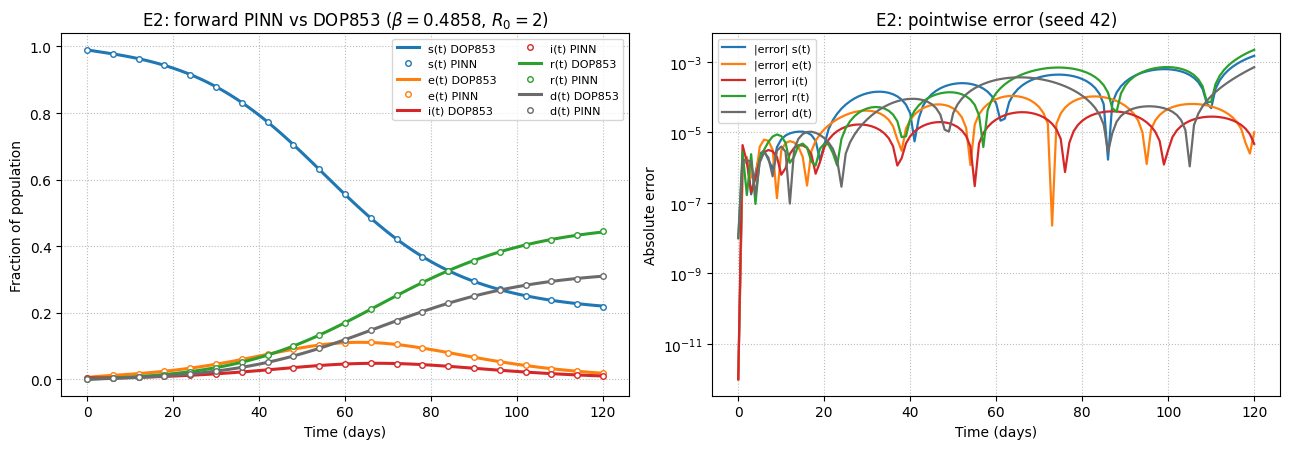
\includegraphics[height=0.28\textheight]{figs/fig_e2_forward_pinn.png}\\
  {\scriptsize\color{mvMuted} E2: forward PINN (markers) vs.\ DOP853 (lines) and pointwise error}\\[4pt]
  \scriptsize\setlength{\tabcolsep}{3pt}
  \begin{tabular}{@{}lcc@{}}
    \toprule
    Quantity & 1\% noise & 5\% noise \\
    \midrule
    $\beta(t)$ rel.\ $L_2$ & $11.0\%\pm0.7\%$ & $11.6\%\pm0.6\%$ \\
    $\mu$ rel.\ error       & $4.6\%\pm0.3\%$  & $5.4\%\pm1.0\%$  \\
    hidden $s(t)$           & $0.36\%\pm0.03\%$ & $0.46\%\pm0.09\%$ \\
    hidden $e(t)$           & $5.8\%\pm0.6\%$   & $6.4\%\pm0.7\%$  \\
    hidden $i(t)$           & $5.8\%\pm0.4\%$   & $6.5\%\pm0.8\%$  \\
    \bottomrule
  \end{tabular}\\[1pt]
  {\tiny\color{mvMuted} E3/E4: mean $\pm$ SD over 5 seeds; $\beta$ drops 0.55$\to$0.25 at day 30}
\column{0.48\textwidth}
  \centering
  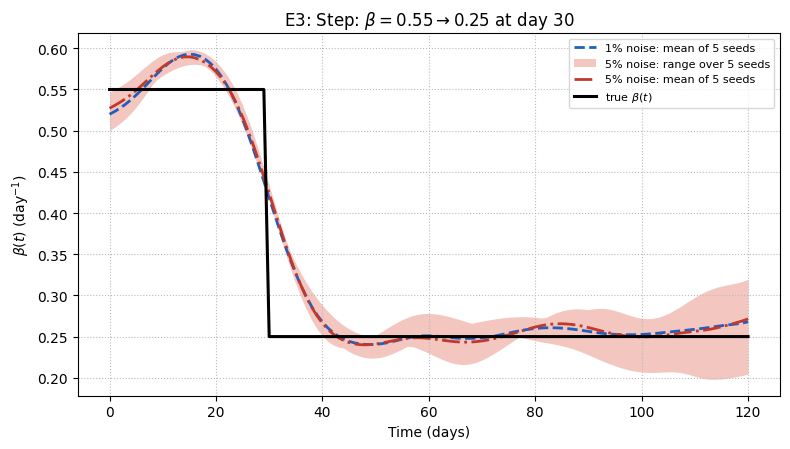
\includegraphics[height=0.28\textheight]{figs/fig_e3_inverse_beta.png}\\
  {\scriptsize\color{mvMuted} E3: recovered $\beta(t)$ (band = seed range, 5\% noise)}\\[2pt]
  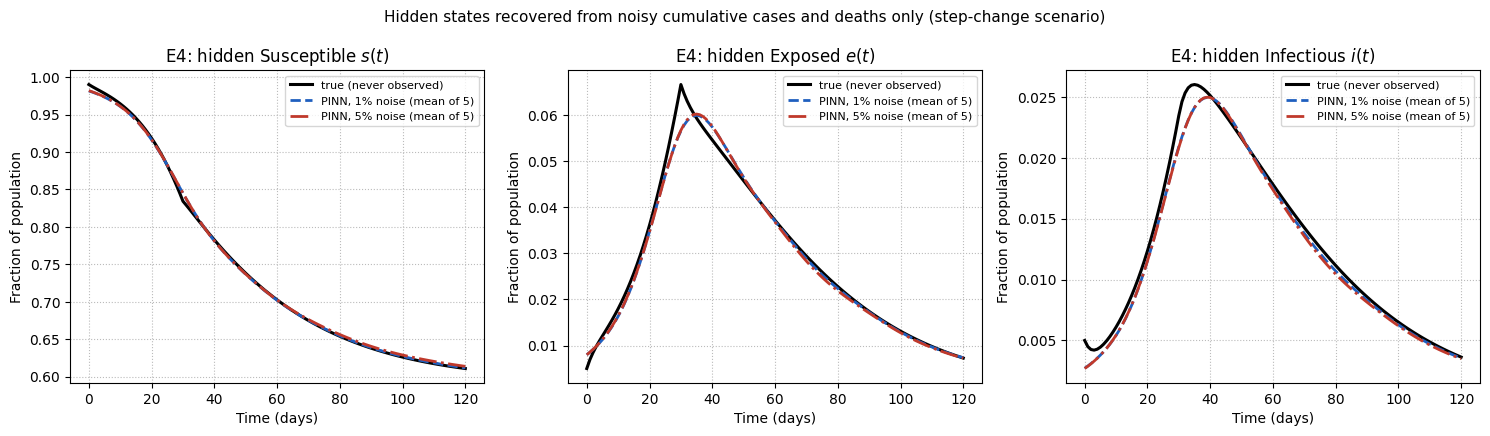
\includegraphics[height=0.28\textheight]{figs/fig_e4_hidden_states.png}\\
  {\scriptsize\color{mvMuted} E4: reconstructed $s(t)$, $e(t)$, $i(t)$ from cases and deaths only}
\end{columns}
\vspace{1pt}
\mvTakeaway{\textbf{E2:} worst compartment $< 2\times10^{-3}$; conservation $2\times10^{-16}$ (machine zero).
\textbf{E3:} a sharp $\beta$ change recovered within 11\%; $5\times$ more noise costs $<1$ pp.
\textbf{E4:} susceptible fraction recovered within $0.5\%$ from \emph{zero} direct measurements.}
\end{frame}
 is needed.
%
% VIDEO NOTE: To embed the PINN training video, place
%   pinn_fitting.mp4  (the uploaded file)  next to this .tex file and
%   uncomment the \movie{}{} frame below before compiling with pdflatex.
%   Acrobat Reader / Foxit are required to play embedded video.
%
\documentclass[aspectratio=169,10pt]{beamer}
\usepackage{graphicx,booktabs,amssymb}
\usepackage{tikz}
\usetikzlibrary{arrows.meta,positioning}
\usepackage{multimedia}   % for \movie{}{} video embed

% ── Beamer theme (identical to Module 1 and Module 5) ───────────────────
\usetheme{default}
\setbeamertemplate{navigation symbols}{}
\definecolor{deckInk}{HTML}{1F2933}
\definecolor{deckAccent}{HTML}{7B2D8E}
\setbeamercolor{frametitle}{fg=deckInk}
\setbeamercolor{framesubtitle}{fg=deckInk!60}
\setbeamercolor{structure}{fg=deckAccent}
\setbeamerfont{frametitle}{series=\bfseries,size=\large}
\setbeamerfont{framesubtitle}{size=\scriptsize}
\setbeamertemplate{frametitle}{%
  \vspace*{4pt}\insertframetitle\par
  {\usebeamerfont{framesubtitle}\usebeamercolor[fg]{framesubtitle}\insertframesubtitle\par}
  \vskip3pt{\color{deckAccent}\hrule height 0.6pt}\vskip-4pt}
\setbeamertemplate{footline}{\hfill{\scriptsize\color{deckInk!50}\insertframenumber}\hspace*{10pt}\vspace*{6pt}}
\setbeamersize{text margin left=18pt,text margin right=18pt}
% ────────────────────────────────────────────────────────────────────────

\begin{document}

% ── Module 4 content frames ─────────────────────────────────────────────
% ======================================================================
% Module 4: Physics-Informed Neural Networks (PINN) for SEIRD
% Three frames, no title slide: \input this file into the main deck.
%
% Needs in the main preamble:
%   \usepackage{graphicx,booktabs,amssymb,multimedia}
%   \usetikzlibrary{arrows.meta,positioning}
% Figures are in figs/ next to this file. If this file sits in a folder
% (e.g. module4/), add \graphicspath{{module4/}} to the main preamble.
% All numbers are from report/main.tex (final Colab run).
% ======================================================================

% Shared deck colours (same values as Module 1 and Module 5)
\definecolor{mvPINN}{HTML}{7B2D8E}
\definecolor{mvPW}{HTML}{2A9D3A}
\definecolor{mvCB}{HTML}{1F5FBF}
\definecolor{mvInk}{HTML}{1F2933}
\definecolor{mvMuted}{HTML}{5F6B7A}
\definecolor{mvSoft}{HTML}{F3EDF6}
\definecolor{mvRule}{HTML}{C9B6D3}

\providecommand{\mvTakeaway}[1]{%
  \par\vspace{3pt}\noindent
  \fcolorbox{mvRule}{mvSoft}{\parbox{\dimexpr\linewidth-2\fboxsep-2\fboxrule\relax}{\footnotesize\color{mvInk}#1}}}

% -----------------------------------------------------------------------
\begin{frame}{PINN design: architecture and inductive biases}
\framesubtitle{Module 4 \textbullet\ two networks share one physics loss \textbullet\ six design choices enforce SEIRD structure exactly}
\vspace{-2pt}
\begin{columns}[T,onlytextwidth]
\column{0.50\textwidth}
  \footnotesize\raggedright
  \textbf{\color{mvPINN}The observability problem}
  \begin{itemize}\setlength{\itemsep}{1pt}
    \item Surveillance reports two series: cumulative cases $C$ and deaths $D$
    \item Hidden compartments $S,E,I$ are \textbf{never measured}
    \item $\beta(t)$ and $\mu$ must be inferred from $C$ and $D$ alone
  \end{itemize}
  \vspace{3pt}
  \textbf{\color{mvPINN}Observable re-parameterisation}\\[1pt]
  {\small Set $C = I+R+D$ (everything symptomatic). Then $S = N-E-C$ exactly, so mass conservation \emph{cannot be violated} for any network output.}
  \vspace{3pt}
  \textbf{\color{mvPINN}Dual-network architecture}
  \begin{itemize}\setlength{\itemsep}{1pt}
    \item \textbf{State net} $g_\theta(\tau)$: $3\times48$ $\tanh$ units, 4 outputs
    \[
      e = e_0\,e^{\tau g_1},\; i = i_0\,e^{\tau g_2},\; c = c_0\,e^{\tau g_3},\; d = d_0+\tau g_4
    \]
    \item \textbf{Transmission net} $h_\phi(\tau)$: $3\times32$ $\tanh$ units,\\ $\beta(\tau)=\operatorname{Softplus}(h_\phi(\tau)+b)>0$
  \end{itemize}
\column{0.47\textwidth}
  \footnotesize\raggedright
  \textbf{\color{mvPINN}Six inductive biases}
  \begin{enumerate}\setlength{\itemsep}{1pt}
    \item \textbf{Hard ICs:} exponential form $e_0 e^{\tau g_1}$ satisfies $e(0)=e_0$ exactly; $\tau$ factor means the gradient of the IC loss is always zero
    \item \textbf{Positivity:} Softplus and exponential forms keep every state $>0$
    \item \textbf{CFR bounds:} $\mu = \gamma\operatorname{CFR}/(1-\operatorname{CFR})$,\; $\operatorname{CFR}\in(0.2,0.8)$, blocks the degenerate $\mu\to 0$ solution
    \item \textbf{Fourier features:} $\sin(k\pi\tau')$ and $\cos(k\pi\tau')$, $k=1,\ldots,4$ overcome spectral bias so $\beta(t)$ changes can be represented inside the window
    \item \textbf{Relative ODE residuals:} each equation divided by its state, so the early (small) phase costs as much as the late (large) phase
    \item \textbf{Smooth prior on $\beta$:} penalty on $(d\beta/d\tau)^2$ makes the inverse problem well-posed
  \end{enumerate}
\end{columns}
\mvTakeaway{\textbf{What the architecture guarantees without training:} $S+E+I+R+D=N$ to machine precision; $e,i,c>0$; initial conditions exact; $\operatorname{CFR}\in(0.2,0.8)$.}
\end{frame}

% -----------------------------------------------------------------------
\begin{frame}{Loss function and training protocol}
\framesubtitle{Module 4 \textbullet\ four terms; Adam brings it close, L-BFGS closes the gap}
\vspace{-2pt}
\begin{columns}[T,onlytextwidth]
\column{0.52\textwidth}
  \footnotesize\raggedright
  \textbf{\color{mvPINN}Total loss}
  \[
    \mathcal{L} = \underbrace{\mathcal{L}_C + \mathcal{L}_D}_{\text{data}} + \mathcal{L}_{\text{ode}} + w_{\text{sm}}\,\mathcal{L}_{\text{smooth}}
  \]
  \vspace{-6pt}
  \begin{align*}
    \mathcal{L}_C &= \tfrac{1}{n_C}\textstyle\sum_k\bigl(c(\tau_k)-C_k/K\bigr)^2 \\
    \mathcal{L}_D &= \tfrac{1}{n_D}\textstyle\sum_k\bigl(d(\tau_k)-D_k/K\bigr)^2 \\
    \mathcal{L}_{\text{ode}} &= \tfrac{1}{N_f}\textstyle\sum_j\Bigl[
      \Bigl(\tfrac{e'-Tf_e}{e}\Bigr)^2\!+\!\Bigl(\tfrac{i'-Tf_i}{i}\Bigr)^2
      \!+\!\cdots\Bigr]_{\!\tau_j} \\
    \mathcal{L}_{\text{smooth}} &= \tfrac{1}{N_f}\textstyle\sum_j\bigl(\tfrac{d\beta}{d\tau}(\tau_j)\bigr)^2
  \end{align*}
  {\scriptsize $K$ = max training case count; $N_f=200$ collocation points; $w_{\text{sm}}=10^{-4}$ (synthetic), $10^{-3}$ (real data); $w_{\text{data}}=w_{\text{ode}}=1$.}
  \vspace{3pt}
  \textbf{\color{mvPINN}Why relative ODE residuals?}\\
  {\small An epidemic grows by orders of magnitude. With plain (absolute) residuals the early phase costs almost nothing. The E6 ablation shows absolute residuals give 75--128\% forward error vs.\ below $2\times10^{-3}$ with relative residuals.}
\column{0.45\textwidth}
  \footnotesize\raggedright
  \textbf{\color{mvPINN}Two-stage optimiser}
  \begin{itemize}\setlength{\itemsep}{1pt}
    \item \textbf{Stage 1 -- Adam} (LR $2\times10^{-3}$, cosine decay, 2000 iters): fresh random collocation points each iteration; fast escape from saddle points
    \item \textbf{Stage 2 -- L-BFGS} (strong-Wolfe line search, 2500--6000 iters, fixed linspace grid): second-order convergence to a tight solution
    \item All weights in \textbf{double precision} (float64) for accurate physics residuals
    \item \textbf{Ensemble:} 5 independent seeds; median is the point estimate
  \end{itemize}
  \vspace{4pt}
  \textbf{\color{mvPINN}Forecasting}\\
  {\small Hold $\beta$ at its mean over the last 14 training days; keep learned $\mu$; integrate forward with DOP853. Forecast is the median over seeds. The assumption that $\beta$ stays constant limits predictive horizon.}
  \vspace{4pt}
  \textbf{\color{mvMuted}E6 ablation headline}\\
  {\small Adam-only: $e(t)$ error $96\%$; $w_{\text{ode}}=10$: errors triple; no Fourier features: $\beta$ RMSE $+38\%$.}
\end{columns}
\mvTakeaway{\textbf{Key design decision:} the L-BFGS stage is non-negotiable. Without it the inverse problem ($\beta(t)$ recovery) barely converges.}
\end{frame}

% -----------------------------------------------------------------------
\begin{frame}{Synthetic experiments: E2 forward, E3 inverse $\beta(t)$, E4 hidden states}
\framesubtitle{Module 4 \textbullet\ no real data; ground truth is known; PINN is tested against DOP853}
\vspace{-4pt}
\begin{columns}[T,onlytextwidth]
\column{0.50\textwidth}
  \centering
  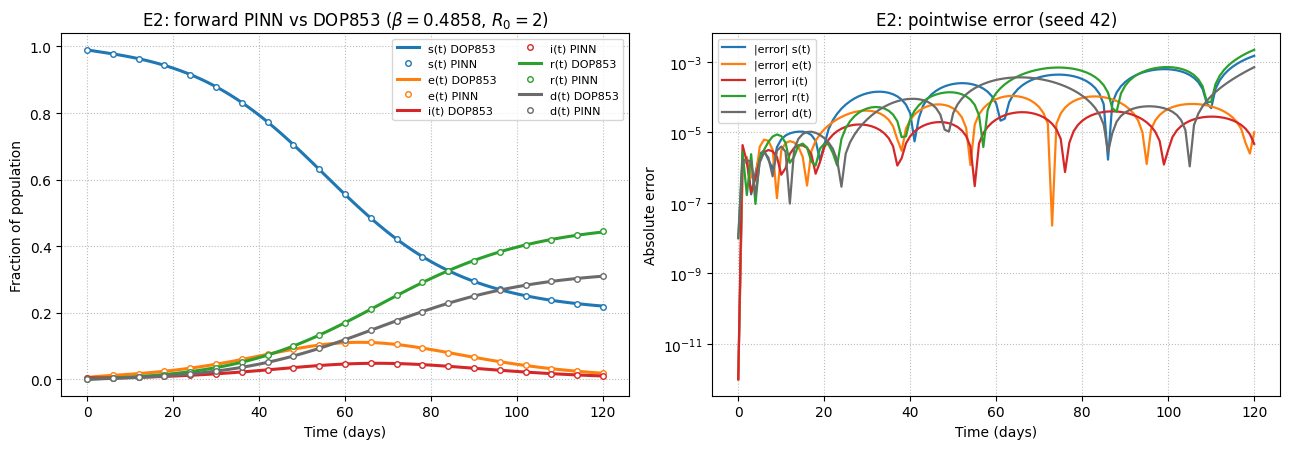
\includegraphics[height=0.28\textheight]{figs/fig_e2_forward_pinn.png}\\
  {\scriptsize\color{mvMuted} E2: forward PINN (markers) vs.\ DOP853 (lines) and pointwise error}\\[4pt]
  \scriptsize\setlength{\tabcolsep}{3pt}
  \begin{tabular}{@{}lcc@{}}
    \toprule
    Quantity & 1\% noise & 5\% noise \\
    \midrule
    $\beta(t)$ rel.\ $L_2$ & $11.0\%\pm0.7\%$ & $11.6\%\pm0.6\%$ \\
    $\mu$ rel.\ error       & $4.6\%\pm0.3\%$  & $5.4\%\pm1.0\%$  \\
    hidden $s(t)$           & $0.36\%\pm0.03\%$ & $0.46\%\pm0.09\%$ \\
    hidden $e(t)$           & $5.8\%\pm0.6\%$   & $6.4\%\pm0.7\%$  \\
    hidden $i(t)$           & $5.8\%\pm0.4\%$   & $6.5\%\pm0.8\%$  \\
    \bottomrule
  \end{tabular}\\[1pt]
  {\tiny\color{mvMuted} E3/E4: mean $\pm$ SD over 5 seeds; $\beta$ drops 0.55$\to$0.25 at day 30}
\column{0.48\textwidth}
  \centering
  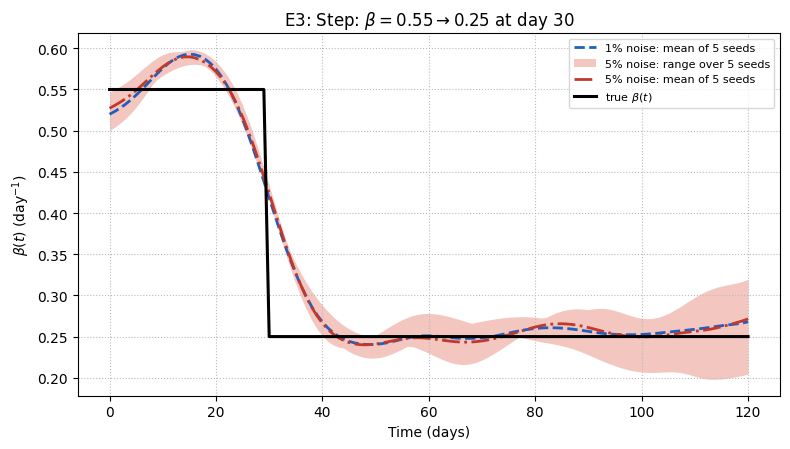
\includegraphics[height=0.28\textheight]{figs/fig_e3_inverse_beta.png}\\
  {\scriptsize\color{mvMuted} E3: recovered $\beta(t)$ (band = seed range, 5\% noise)}\\[2pt]
  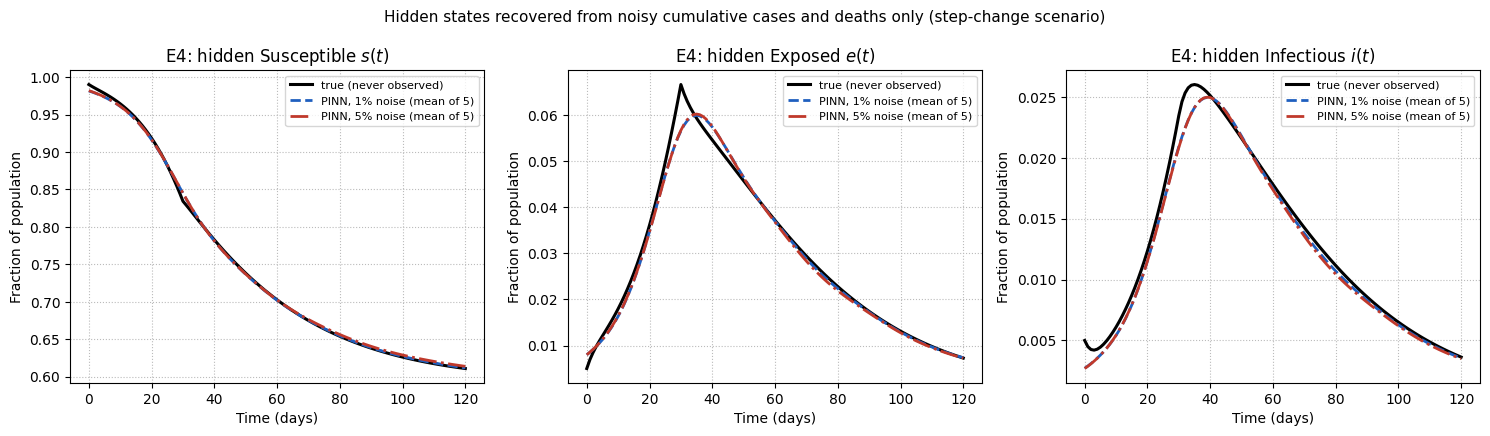
\includegraphics[height=0.28\textheight]{figs/fig_e4_hidden_states.png}\\
  {\scriptsize\color{mvMuted} E4: reconstructed $s(t)$, $e(t)$, $i(t)$ from cases and deaths only}
\end{columns}
\vspace{1pt}
\mvTakeaway{\textbf{E2:} worst compartment $< 2\times10^{-3}$; conservation $2\times10^{-16}$ (machine zero).
\textbf{E3:} a sharp $\beta$ change recovered within 11\%; $5\times$ more noise costs $<1$ pp.
\textbf{E4:} susceptible fraction recovered within $0.5\%$ from \emph{zero} direct measurements.}
\end{frame}


% ── Optional video frame (uncomment if pinn_fitting.mp4 is present) ─────
%
% \begin{frame}{PINN fitting in action}
% \framesubtitle{Module 4 \textbullet\ Adam + L-BFGS convergence on the E3 inverse problem}
% \centering
% \movie[width=0.85\textwidth,height=0.60\textheight,poster,showcontrols,autostart]{%
%   \includegraphics[width=0.85\textwidth,height=0.60\textheight,keepaspectratio]%
%   {figs/fig_e2_forward_pinn.png}%
% }{pinn_fitting.mp4}
% \end{frame}

\end{document}
